\section{The navigator}
\label{sec:navigator}
A navigator must be able to create a huge metaverse and democratize
its use. For this reason, we base our navigator on the Ogre 3D
rendering engine. Its robustness, efficiency,
upgradability and openness  are, in fact, essential features for a durable
system. Moreover, Ogre 3D can be easily embedded in web pages thanks
to a Mozilla or ActiveX plugin. Conversely, web pages can be mapped
on 3D models as interactive textures thanks to the Navi library based
on Gecko. Thus, the navigator allows a Web 2.0 navigation inside the
Web 3D, as well as a Web 3D navigation inside the Web 2.0. Our view
is, in fact, that Web 3D and Web 2.0 should integrate each other (see figure
\ref{Fig:navigator}).
\begin{figure}
\center
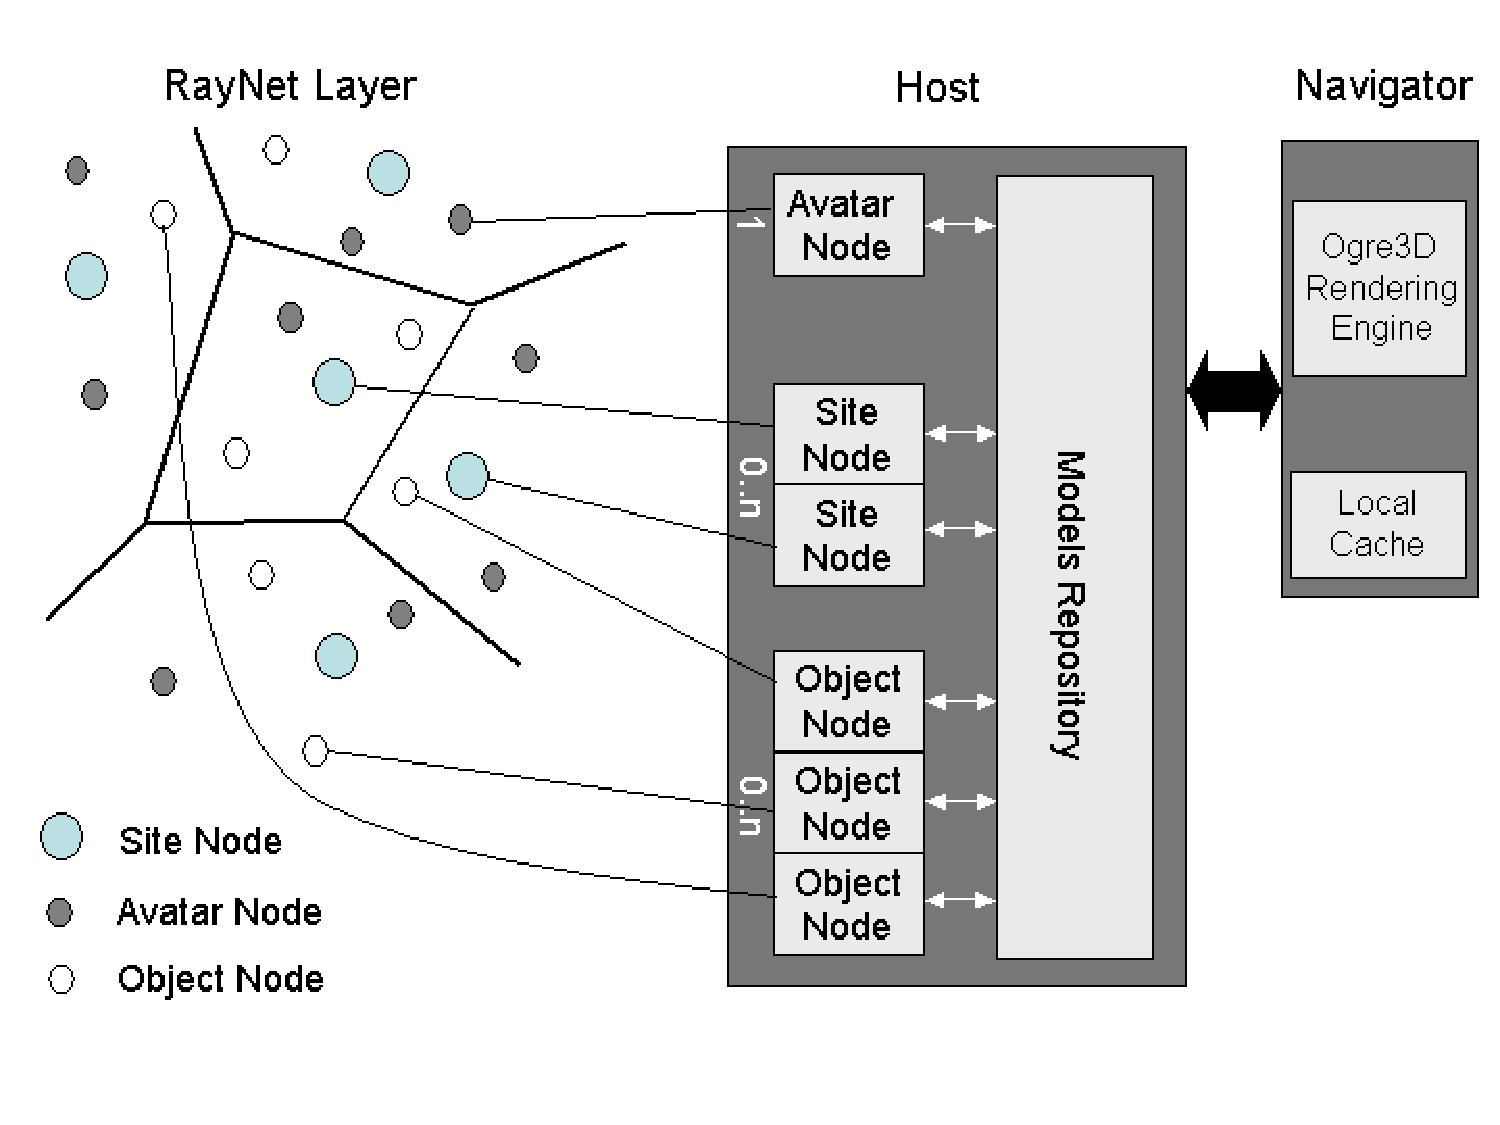
\includegraphics[width=3in]{Figures/host.pdf}
\vspace{-3ex}
\fcaption{Nodes hosted on a proxy server to allow accesses to the metaverse on terminals with low resources such as mobiles.}
\label{Fig:host}
\end{figure}
\begin{figure}[!t]
\center
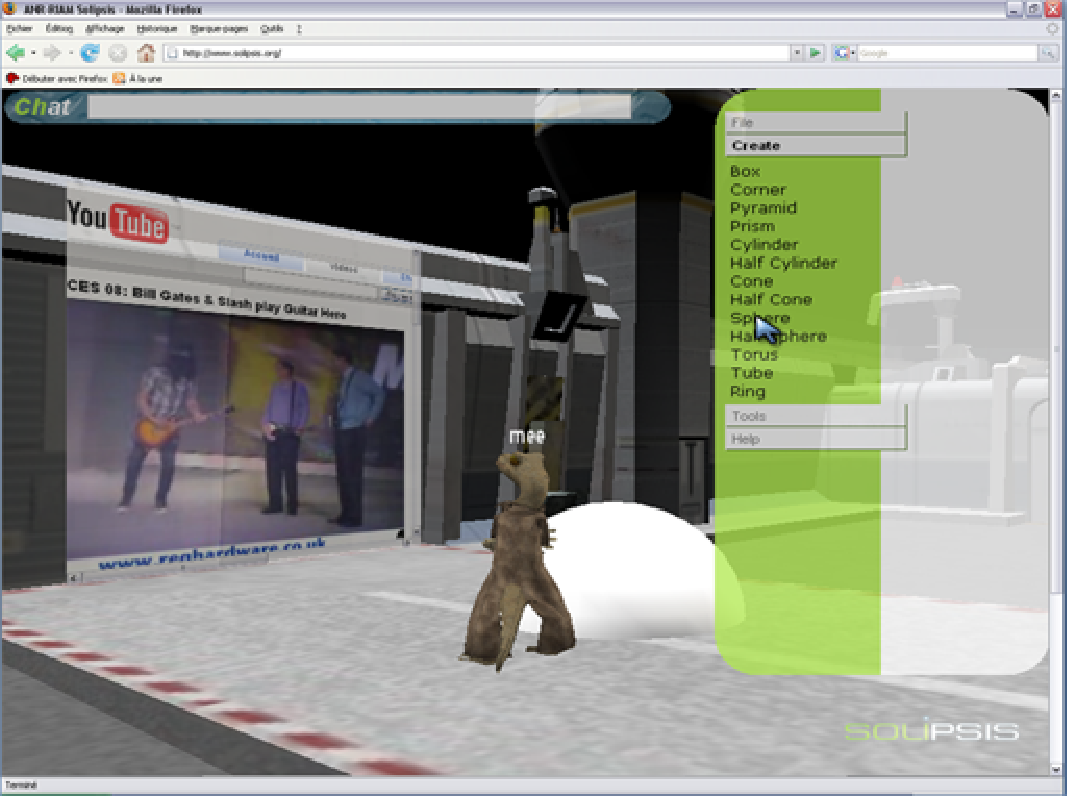
\includegraphics[width=2.7in]{Figures/navigator.pdf}
%\vspace{-2ex}
\fcaption{Web based navigator embedding modeling tools, and providing a mapping of web pages as interactive textures.}
\label{Fig:navigator}
\end{figure}
Since the vitual universe belongs to all users, modeling tools are
embedded within the navigator in order to create, modify or delete
contents. At the moment, we focus on intuitive tools, but procedural,
declarative, parametric and sketch-based modeling tools are obviously
considered. Finally, to provide access to the virtual universe on
mobile devices, nodes can be hosted by proxy servers, to reduce the
amount of computation that has to be performed on terminals with
scarce resources. Thus, hosts can compute collision detection, physics
animation, data-exchange management, and viewpoint-based filtering,
and then communicate with the navigator that only needs to render the
virtual environment and interact with it (see figure \ref{Fig:host}).
